
\subsubsection{Задача $topN$}
Как говорилось во введении первой главы, правила вывода АКМ
основываются на эвристических утверждениях. Приведем эвристическое утверждение,
на котором базируется правило вывода $\Pi$ ООМ (далее это правило будем
обозначать $\Pi_O$), использующееся для решения
задачи $topN$ \cite{item-based,topn1,amazon-item2item}:
\begin{assert}\label{assertORS1}
Если пользователю нравится объект $i$, который
похож на объект $j$, то пользователю понравится объект $j$.
\end{assert}

Во введенной
терминологии данное утверждение примет следующий вид:
\begin{equation}
\label{ors-assert}
(u_a \R i) \wedge (i \rt j) \Rightarrow u_a \R j,
\end{equation}
где формально неопределенные термины, использующиеся в существующих
исследованиях, заменены на формальные обозначения.

На Рисунке \ref{amazon-ex1} приведен пример работы
сервиса LastFm, который иллюстрирует
работу РС при использовании правила вывода $\Pi_O$, основанного на утверждении
(\ref{assertORS1}): РС рекомендует пользователю музыкальных исполнителей,
между которыми и искомым выполняется отношение близости.

\begin{figure}[htb]
	\caption{Пример рекомендации сервиса LastFm. Искомый исполнитель ---
\textquotedblleft Pink Floyd \textquotedblright, снизу --- схожие исполнители}
\begin{center}
	\label{amazon-ex1}
 
\includegraphics[width=7in,height=7in]{pics/lstfm-rs-example.jpeg}
\end{center}
\end{figure}

В момент решения задачи $topN$ и в момент проверки качества решения
в ООМ используется информация только
о тех объектах, для которых известно, что $(u_a \R i_0) \wedge (u_a \R
i_{\bot})$\footnote{
	Во-первых, данная информация является достаточной для решения задачи
	$topN$, а, во-вторых, информация о других значениях $\rho(u, i)$
	может быть недоступна. К примеру, для случая интернет-магазина, где
	существует только факт наличия приобретения товара без его оценки.
	},
поэтому при решении задачи $topN$ будем работать с множеством исходных
данных вида $P = \{(u, i, \rho(u, i)): u \R i \}$.

Правило вывода $\Pi_O$ ООМ для решения задачи $topN$ задается следующей формулой:
\begin{equation}
	\label{ors-pi-top}
	i \rt i_0 \Rightarrow (\rh(u_a, i) := 1) \wedge (u_a \R i)
\end{equation}
Значения $\rh(u_a, i)$ задаются равными единице, потому что тогда объекты $i$
будут близкими для активного пользователя при любом пороговом значении
$\Delta_{\R}$.
Правило вывода $\Pi_O$ говорит о том,
что если существует объект $i$, являющийся соседом для объекта $i_0$,
то, следуя эвристическому утверждению модели (\ref{assertORS1}), выполняется
отношение $u_a \R i$,
так как $u_a \R i_0$ по принятому для задачи $topN$ виду исходного множества.
То есть решение можно записать в форме утверждения: $(u_a \R i_0) \wedge (i \rt
i_0) \Rightarrow u_a \R i$.

Приведем схему решения задачи $topN$ при использовании правила вывода $\Pi_O$
(\ref{ors-pi-top}). Для того, чтобы составить множество объектов, между которыми и
активным пользователем выполняется отношение близости, по правилу вывода нужно найти объекты,
между которыми и объектами обучающего множества будет выполняться отношение
близости. Тогда, следуя эвристическому утверждению, между найденными объектами
и активным пользователем будет выполняться отношение близости: пусть $i \rt
i_0$, тогда, так как по виду исходного множества, принятого для задачи $topN$
выполняется $u_a \R i_0$, по эвристическому утверждению (\ref{assertORS1})
выполняется $u_a \rt i$ ---
$(u_a \R i_0) \wedge
(i \rt i_0) \Rightarrow u_a \rt i$, --- что и требуется по задаче $topN$.

Схему решения задачи $topN$ можно описать как формирование кластера
объектов $\nit = \{ i : i \rt I^a_0 \}$,
$|\nit| = N$, где
$I^a_0 = \{i_0: \rho(u_a, i_0) \in P_0\}$ --- центр кластера. Множество
объектов кластера (кроме центра) является искомым решением.

Определим способы задания отношения близости между объектом $i$ и
подмножеством объектов $I^a_0$
\label{deltaTneighbours}
 \cite{topn1,topn2,amazon-item2item,disser0}:
\begin{itemize}
	\item $I^a_0 \rt i \Leftrightarrow \Bigr( \frac{1}{|I^a_0|} \cdot \sum \limits_{i_0
		\in I^a_0} \di(i,i_0) \Bigl) \ge \Delta_i$.
		В стандартном решении  \cite{item-based} $topN$
		для определения меры близости между объектом $i$ и множеством объектов
		$I^a_0$ вычисляется сумма мер близости между объектом $i$ и объектами
		$i_0 \in I^a_0$.
		$I^a_0 \rt i \Rightarrow \Bigr( \frac{1}{|I^a_0|} \cdot \sum \limits_{I^a_0 \in I^a_0}
		\di(i,I^a_0)\Bigl) \ge \Delta_i \Rightarrow \exists$
$i_0 \in I^a_0, I^a_0 \rt i$.
По данным задачи и вследствие выполнения отношения $I^a_0 \rt i$, выполняется
		$(u_a \R I^a_0) \wedge (I^a_0 \R i) \Rightarrow u_a \R i$. Таким образом,
если объект $i$ принадлежит кластеру $\nit$ (то есть выполняется
		$I^a_0 \rt i$), то по утверждению ООМ  (\ref{assertORS1}) выполнится $u_a \R i$.
Поэтому данный способ определения отношения $i \rt I^a_0$ можно
		применять с правилом вывода $\Pi_O$ (\ref{ors-pi-top}) для решения задачи

\item $I^a_0 \rt i \Leftrightarrow$  $\exists I^a_0 \in I^a_0, I^a_0 \rt i$.
По данным задачи и способу задания $I^a_0 \rt i$ выполняется утверждение ООМ, то есть
		$(u_a \R I^a_0) \wedge (I^a_0 \rt i) \Rightarrow u_a \R i$.

Таким образом, если объект $i$ принадлежит кластеру $\nit$ (то есть $I^a_0 \rt i$),
		то по утверждению ООМ (\ref{assertORS1}) выполнится $u_a \R i$, что и требуется
от задачи.
Поэтому данный способ определения отношения $i \rt I^a_0$ можно
		применять с правилом вывода $\Pi_O$ (\ref{ors-pi-top}) для решения задачи
$topN$.
\end{itemize}
%%% Для вычисления значения меры близости между объектами системы может использоваться самая различная информация об объектах, которая
%%% зависит от реализации и предметной области РС\footnote{Поэтому при описании схемы, как 
%%% правило, не уделяется внимание контентам объектов}. К примеру, для кинематографической РС сценарий рекомендаций можно описать так: 
%%% если пользователь приобрел коллекцию DVD <<Крестный отец>>, то система может произвести рекомендации тех DVD, 
%%% где участвует Марлон Брандо, режиссером которых является Френсис Форд Коппола, или в жанре криминальная драма. 
%%% То есть характеристиками объекта может выступать любая
%%% известная и значительная информация о нем, в данном случае это: известный актер, режиссер и жанр.
%%--------------------------------------------
\bigbreak
Опишем один из вариантов исполнения ООМ и решим
задачу $topN$  \cite{item-based}.%TODO: set cite
\begin{itemize}
	\item $c_X(u_a) = (x_1, x_2, ..., x_|I|)$
		\begin{equation*}
			x_i =
			\begin{cases}
				1, &\text{если $u_a \R i$}\\
				0, &\text{иначе}
			\end{cases}
		\end{equation*}
		контент активного пользователя --- вектор {\it бинарных} оценок,
		отображающий информацию о том, какие объекты пользователь предпочитает.
		Примером такого контента является контент пользователя
		РС Amazon \cite{amazon-item2item}, где $x_i = 1$ означает то, что пользователь
		приобрел товар $i$;
	\item контент объекта в исследованиях РС, как правило,
		не определяется, так как множество характеристик объектов,
		их значений и структура контента не влияют на технику решения и могут
		варьироваться для различных реализаций РС. В описываемой модели
		воспользуемся векторным представлением, то есть
		$c_Y = (y_1,...,y_{|Y|})$;
	\item
		$\di(i,j) =\cos(\angle(c_Y(i),c_Y(j)))$.

		Типичной мерой близости, используемой при решении задачи $topN$ является
		косинус угла между контентами объектов, представляемых в виде векторов
		\cite{item-based,rs-handbook}.
	\item
		Чтобы не производить расчеты меры близости при формировании
		$\overline{P}^a_{\bot}$ каждый раз, когда активный пользователь
		делает запрос на решение задачи $topN$, значения мер близости $\di$
		рассчитываются заранее и заносятся в специальную матрицу $\mathbb{M}$
		размера $|I| \times |I|$:
		\begin{equation*}
			\mathbb{M}_{ij} =
			\begin{cases}
				\di(i,j), & i \ne j \\
				0, & \text{иначе}
			\end{cases}
		\end{equation*}

		Такой предварительный этап называется построением модели \cite{topn2}.
\end{itemize}

На рисунке (\ref{dia:matrix}) изображена блок-схема алгоритма
построения матрицы $\mathcal{M}$, которой соответствует псевдокод, представленный на изображении <<Алгоритм построения матрицы мер близости объектов>>  (\ref{alg:matrix})
\begin{figure}[htb]
	\caption{Блок-схема алгоритма построения матрицы $\mathcal{M}$}
\begin{center}
	\label{dia:matrix}
 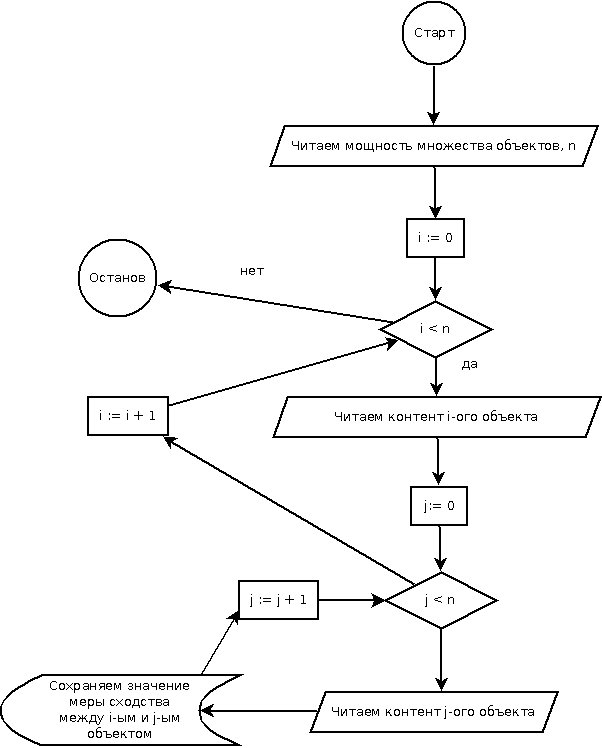
\includegraphics[width=6in,height=7in]{pics/algs/matrix.png}
\end{center}
\end{figure}

%\begin{figure}[htbp]
\begin{figure}[htb]
\caption{Алгоритм построения матрицы мер близости объектов}
\label{alg:matrix}
%\begin{algorithm}
\begin{algorithmic}[1]
\For{$i \gets 1, i \le n$}
	\State $\mathbb{M}_{ii} \gets 0$ \Comment{Чтобы пара с одинаковыми
	объектами не участвовала в дальнейших расчетах}
  \For{$j \gets 1, j \le n$}
  \State $\mathbb{M}_{ij} \gets \di(i,j)$
  \State $\mathbb{M}_{ji} \gets \mathbb{M}_{ij}$
  \State $j \gets j + 1$
  \EndFor
\State $i \gets i + 1$
\EndFor
\end{algorithmic}
%\end{algorithm}
\end{figure}

Для нахождения решения задачи $topN$ построим вектор
$\mathit{M} = (\overline{x}_1,...,\overline{x}_|I|)$, где
$
\overline{x}_i =
\begin{cases}
	0, &\text{если  $i \in I^a_0 $}\\
\mathbb{M}^i \times c_X(u_a)^T, &\text{ иначе }
\end{cases}
$\\
$c_X(u_a)^T$ --- транспонированный контент-вектор активного пользователя.
$I_{topN} = \{ i \in \{\overline{x}_i\} )\}$, где
$\{\overline{x}_i\}$ --- множество, состоящее из $N$ наибольших значений
координат вектора $\mathit{M}$.

На рисунке <<Блок-схема стандартного алгоритма решения задачи $topN$ в ООМ>> (\ref{dia:topn-solve-ors}) изображена блок-схема стандартного
алгоритма алгоритма решения задачи $topN$ в ООМ, которой соответствует
псевдокод, представленный на изображении <<Стандартный метод решения задачи $topN$ в ООМ>> (\ref{alg:topn-solve-ors})
\begin{figure}[htb]
	\caption{Блок-схема стандартного алгоритма решения задачи $topN$ в ООМ}
\begin{center}
	\label{dia:topn-solve-ors}
 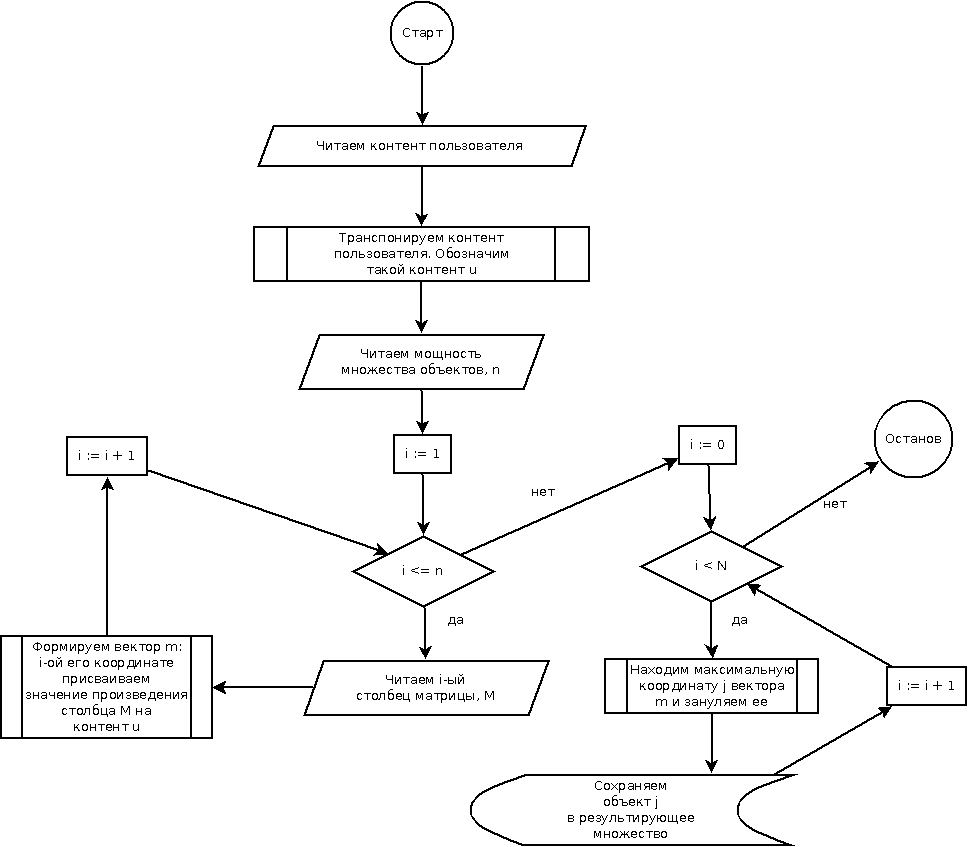
\includegraphics[width=7in,height=8in]{pics/algs/topn-ors.png}
\end{center}
\end{figure}

\begin{figure}[htb]
%\begin{algorithm}
\caption{Стандартный метод решения задачи $topN$ в ООМ}
\label{alg:topn-solve-ors}
\begin{algorithmic}[1]
\For{$i \gets 1, l \le n$} \Comment{Умножаем вектор-контент на матрицу}
	\State $m_i \gets \mathbb{M}^i \times c_X(u_a)^T$
\EndFor
\For{$j \gets 1, j \le N$}
	\State $i \gets \underset{i}{\mathrm{argmax}} \text{ } \overline{x}_i$
	\State $I_{topN} \gets I_{topN} \bigcup \{i\}$
	\Comment{Выбираем координату вектора $\mathit{M}$ с наибольшим значением}
\bigbreak
  \State $\overline{x}_i \gets 0$ \Comment{Зануляем уже выбранную координату}
  \State $j \gets j + 1$
\EndFor
\end{algorithmic}
%\end{algorithm}
\end{figure}
